\documentclass[paper=screen,10pt,unicode]{beamer}
\usepackage[T2A]{fontenc}
\usepackage[utf8]{inputenc}
\usepackage[russian, english]{babel}
\usepackage{tikz}
\usepackage{graphicx}

\mode<presentation>
{
	\usetheme{Frankfurt}
}

\author{Андрей Бреслав \\ \texttt{abreslav@gmail.com}}
\institute[ИТМО]{СПбГУ ИТМО}

\newcommand{\mytitle}{Применение принципов MDD и AOP к разработке ПО, связанного с формальными грамматиками}

\subject{\mytitle}
\AtBeginSection[]
{
	\begin{frame}<beamer>
		\frametitle{Содержание}
		\tableofcontents[currentsection,currentsubsection]
	\end{frame}
}

\title[Grammarware Engineering]{\mytitle}

\date{\today}

\begin{document}

\begin{frame}
	\titlepage
\end{frame}

\begin{frame}
	\frametitle{Содержание}
	\tableofcontents
\end{frame}

\section{Описание проблемы}
\begin{frame}
	\frametitle{ПО, связанное с грамматиками}
	\begin{block}{Приложения}
		\begin{itemize}
			\item Компиляторы
			\item Средства статического анализа кода
			\item Форматы файлов данных
			\item Средства преобразования кода
			\item Средства автоматического документирования
			\item ...
		\end{itemize}
	\end{block}
	\begin{block}{Средства разработки}
		\begin{itemize}
			\item Генераторы компиляторов (интерпретаторов, парсеров)
			\item Генераторы текстовых редакторов с подсветкой
			\item \large \bf\alert{???}
		\end{itemize}
	\end{block}
\end{frame}

\begin{frame}
	\frametitle{Проблемы}

	\begin{block}{С грамматическими определениями очень трудно работать}
		\begin{itemize}
			\item Плохая читаемость
			\item Смешение различных функций
			\item Очень трудно поддерживать
			\item Практически невозможно повторно использовать
			\item Большое количество дублирующейся информации
		\end{itemize}
	\end{block}
	\begin{block}{Результат}
		\begin{itemize}
			\item Многие делают все вручную
			\item Возникает большое количество ошибок
			\item Создание качественного ПО, работающего с грамматиками, затруднено
		\end{itemize}
	\end{block}
\end{frame}

\begin{frame}
	\frametitle{Grammarware Engineering}

	\begin{block}{Основатели подхода}
		Статья P. Klint, R. L\"{a}ammel, C. Verhoef, ``Towards an engineering discipline for GRAMMARWARE'', 2005 год
	\end{block}
	\begin{block}{}
		\alert{Grammarware} -- программы, использующие грамматики или основанные на грамматиках.
	\end{block}
	\begin{block}{Grammarware engineering}
		\begin{itemize}
			\item Шаблоны проектирования
			\item Стандарты
			\item {\bf Специализированные средства разработки }
		\end{itemize}
	\end{block}
\end{frame}

\section{Предлагаемый подход}
\begin{frame}
	\frametitle{Что такое Grammatic}

	\begin{block}{Идея}
		Программное средство для разработки Grammarware, основанное на идеях Model-Driven Development
		и Аспектно-Ориентированного Программирования
	\end{block}
	\begin{block}{Преимущества}
		\begin{itemize}
			\item Разделение аспектов системы
			\item Модульность и повторное исопльзование артефактов разработки
			\item Гибкость при эволюции системы
			\item Выбор конкретной технологии (класс грамматики, платформа и т.д.) на поздних этапах разработки
			\item Автоматизация манипуляций с грамматиками
		\end{itemize}
	\end{block}
\end{frame}

\begin{frame}
	\frametitle{Как этого добиться}

	\begin{block}{Определение грамматики ничем не расширено}
		\begin{itemize}
			\item ``Чистая'' EBNF
			\item Никакого кода семантических действий
			\item Никаких дополнительных ограничений на класс грамматики (LL(k), LALR и т.д.)
		\end{itemize}
	\end{block}
	\begin{block}{Прочие аспекты системы определяются отдельно}
		\begin{itemize}
			\item Проверка грамматики на корректность
			\item Преобразования грамматики
			\item Генерация моделей по грамматике
			\item Генерация кода
			\item ...
		\end{itemize}
	\end{block}
\end{frame}

\begin{frame}
	\frametitle{Реализация}
	\begin{block}{Запросы и преобразования}
		\begin{itemize}
			\item Выбрать из грамматики объекты с заданными свойствами
			\item Преобразовать выбранные объекты
		\end{itemize}
	\end{block}
	\begin{block}{}
		Примеры запросов
		\begin{itemize}
			\item Все нетерминалы, имена которых начинаются на E
			\item Все правила, у которых в правой части по два нетерминала
		\end{itemize}
	\end{block}
	\begin{block}{Преобразования}
		\begin{itemize}
			\item Изменение структуры грамматики
			\item Создание объектов в какой-либо метамодели
			\item Генерация сообщений об ошибках
			\item Генерация текста
		\end{itemize}
	\end{block}
\end{frame}

\section{Система Grammatic}

\begin{frame}
	\frametitle{Архитектура системы}
	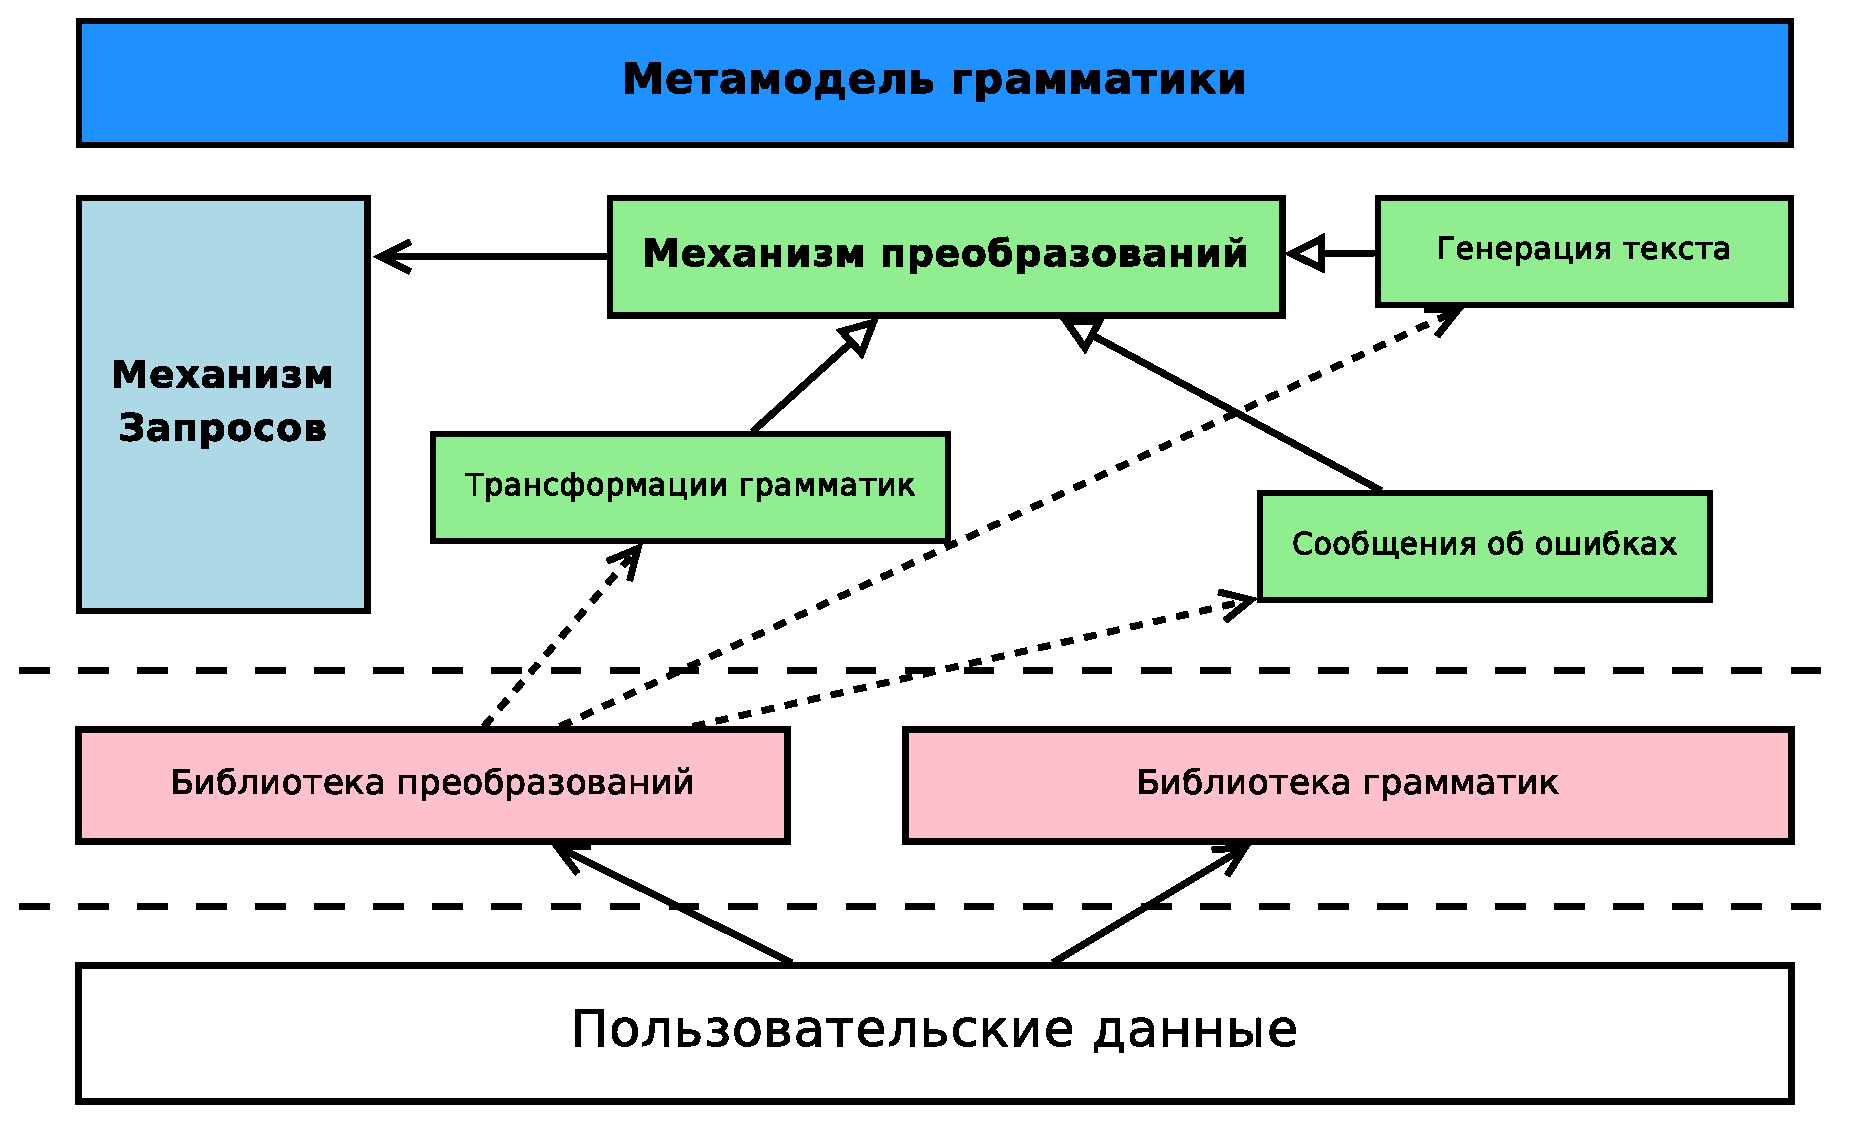
\includegraphics[width=110mm,height=70mm]{grammatic_structure.eps}	
\end{frame}

\begin{frame}
	\frametitle{Общая схема использования}
	\begin{center}
 		\includegraphics[width=100mm,height=70mm]{grammatic_usage.eps}	
	\end{center}
\end{frame}

\begin{frame}
	\frametitle{Пример использования}
	\begin{center}
 		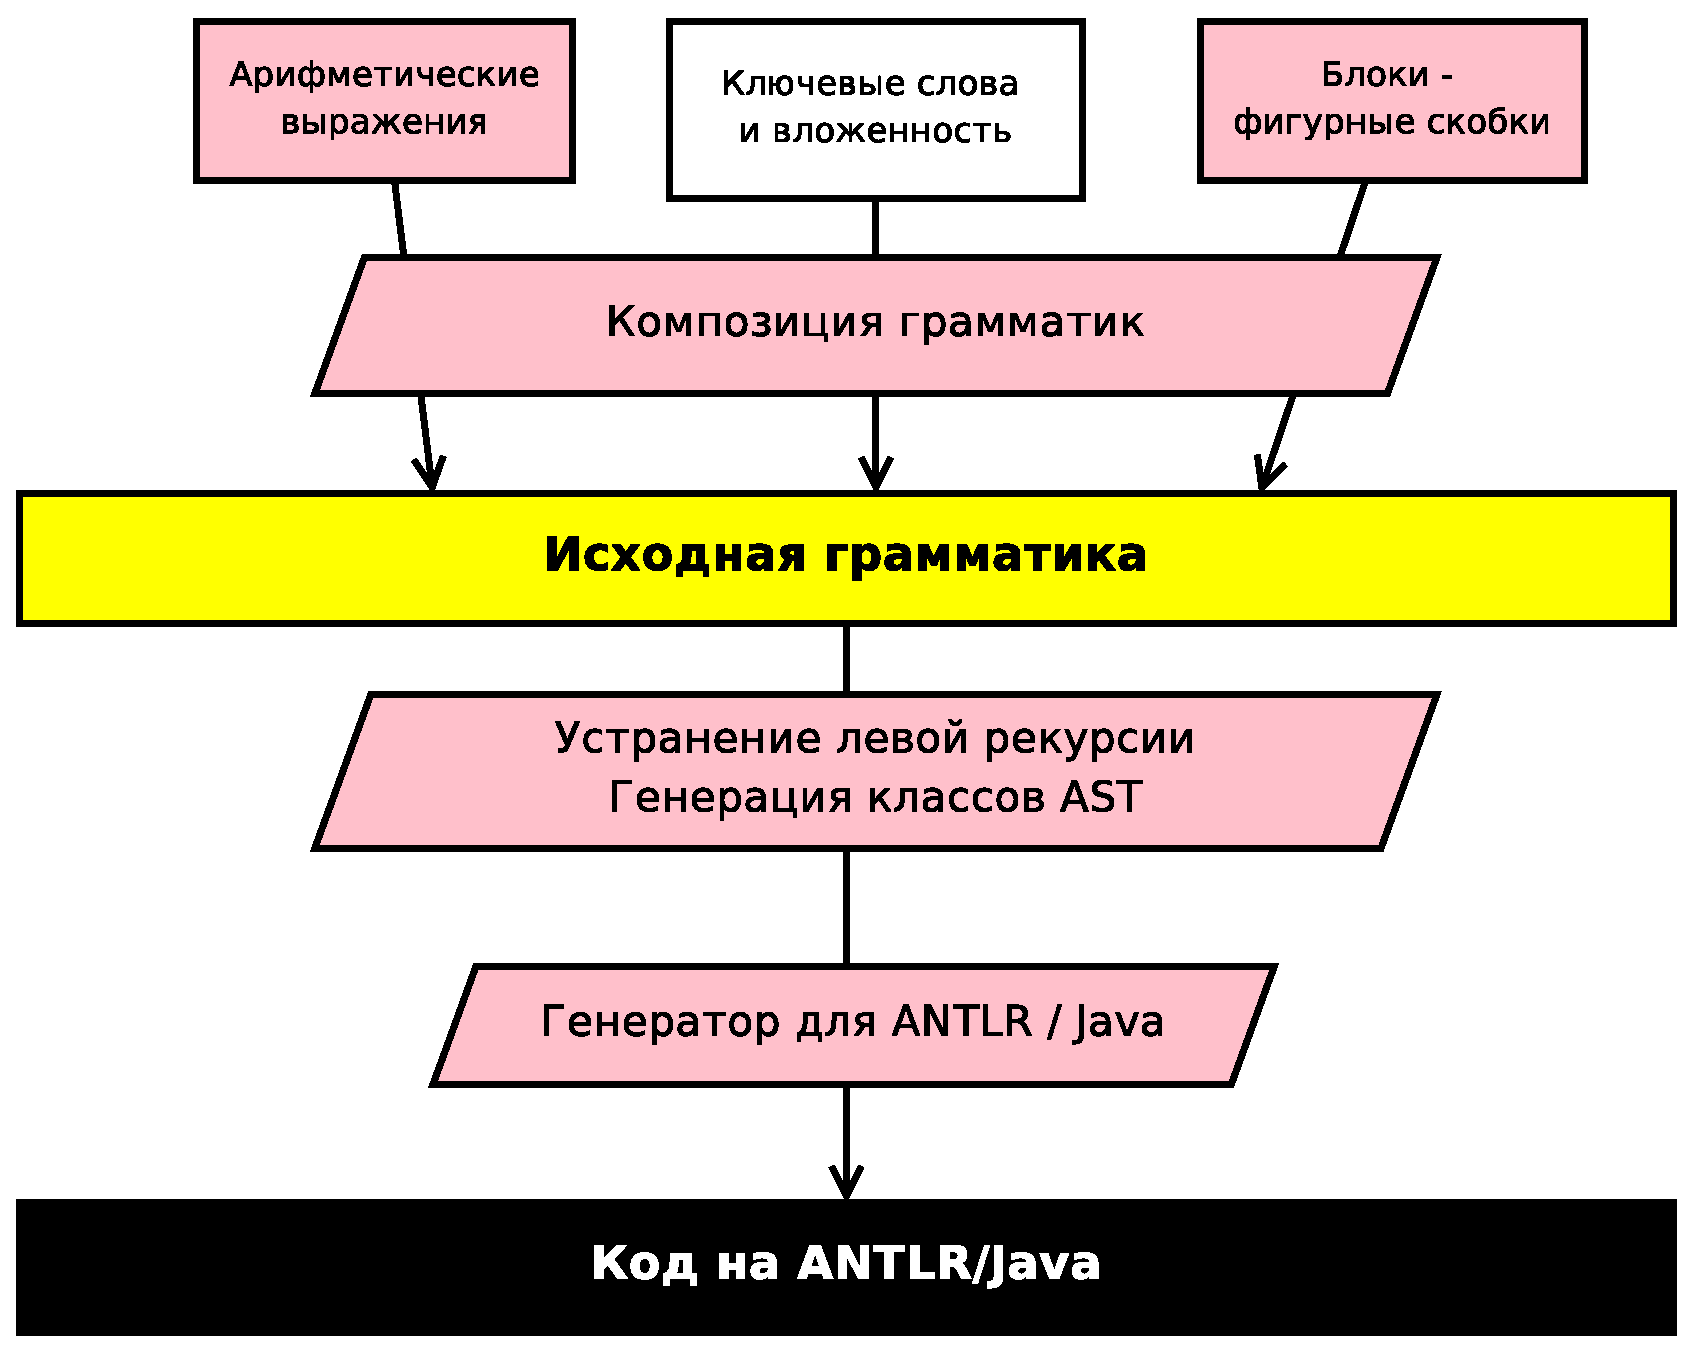
\includegraphics[width=100mm,height=70mm]{grammatic_usage_example.eps}	
	\end{center}
\end{frame}

\begin{frame}
	\frametitle{Области применения}

	\begin{block}{Создание полнофункционального Grammarware}
			\begin{itemize}
				\item Модульность и повторное использование
				\item Легкость эволюции системы
				\item Гибкость при выборе целевой платформы
			\end{itemize}
	\end{block}
	\begin{block}{Прототипирование и создание ПО для внутреннего использования}
			\begin{itemize}
				\item Сборка из крупных блоков в стиле RAD
				\item Возможность использовать наработки при разработке полнофункционального ПО 
			\end{itemize}
	\end{block}
	\begin{block}{Примеры ``разовых'' приложений}
		\begin{itemize}
			\item Предметно-ориентированные языки (DSL)
			\item Средства аудита
			\item Средства миграции с одной библиотеки на другую
		\end{itemize}
	\end{block}
\end{frame}

\section{Платформа для создания инструментов}

\begin{frame}
	\frametitle{Платформа для создания инструментов}

	\begin{block}{Примеры специализированных инструментов}
		\begin{itemize}
			\item Генератор парсеров
			\item Генератор тестов для грамматик
			\item Преобразователь грамматики в UML-диаграмму классов
		\end{itemize}
	\end{block}
	\begin{block}{Составляющие специализированного инструмента}
		\begin{itemize}
			\item Ограничения на структуру грамматики
			\item Ограничения на метаданные
			\item Преобразования грамматики
		\end{itemize}
	\end{block}
	\begin{block}{Вывод}
		Grammatic может стать платформой для создания таких инструментов
	\end{block}
\end{frame}

\section{Вопросы}

\begin{frame}
	\frametitle{Спасибо за внимание!}
	
	Ваши вопросы
\end{frame}

\end{document}

